\documentclass{article}

\usepackage{arxiv}

\usepackage[utf8]{inputenc} % allow utf-8 input
\usepackage[T1]{fontenc}    % use 8-bit T1 fonts
\usepackage{lmodern}        % https://github.com/rstudio/rticles/issues/343
\usepackage{hyperref}       % hyperlinks
\usepackage{url}            % simple URL typesetting
\usepackage{booktabs}       % professional-quality tables
\usepackage{amsfonts}       % blackboard math symbols
\usepackage{nicefrac}       % compact symbols for 1/2, etc.
\usepackage{microtype}      % microtypography
\usepackage{lipsum}
\usepackage{graphicx}

\title{A template for the \emph{arxiv} style}

\author{
    David S. Hippocampus
    \thanks{Use footnote for providing further information about author
(webpage, alternative address)---\emph{not} for acknowledging funding
agencies. Optional.}
   \\
    Department of Computer Science \\
    Cranberry-Lemon University \\
  Pittsburgh, PA 15213 \\
  \texttt{\href{mailto:hippo@cs.cranberry-lemon.edu}{\nolinkurl{hippo@cs.cranberry-lemon.edu}}} \\
   \And
    Elias D. Striatum
   \\
    Department of Electrical Engineering \\
    Mount-Sheikh University \\
  Santa Narimana, Levand \\
  \texttt{\href{mailto:stariate@ee.mount-sheikh.edu}{\nolinkurl{stariate@ee.mount-sheikh.edu}}} \\
  }

\usepackage{color}
\usepackage{fancyvrb}
\newcommand{\VerbBar}{|}
\newcommand{\VERB}{\Verb[commandchars=\\\{\}]}
\DefineVerbatimEnvironment{Highlighting}{Verbatim}{commandchars=\\\{\}}
% Add ',fontsize=\small' for more characters per line
\usepackage{framed}
\definecolor{shadecolor}{RGB}{248,248,248}
\newenvironment{Shaded}{\begin{snugshade}}{\end{snugshade}}
\newcommand{\AlertTok}[1]{\textcolor[rgb]{0.94,0.16,0.16}{#1}}
\newcommand{\AnnotationTok}[1]{\textcolor[rgb]{0.56,0.35,0.01}{\textbf{\textit{#1}}}}
\newcommand{\AttributeTok}[1]{\textcolor[rgb]{0.77,0.63,0.00}{#1}}
\newcommand{\BaseNTok}[1]{\textcolor[rgb]{0.00,0.00,0.81}{#1}}
\newcommand{\BuiltInTok}[1]{#1}
\newcommand{\CharTok}[1]{\textcolor[rgb]{0.31,0.60,0.02}{#1}}
\newcommand{\CommentTok}[1]{\textcolor[rgb]{0.56,0.35,0.01}{\textit{#1}}}
\newcommand{\CommentVarTok}[1]{\textcolor[rgb]{0.56,0.35,0.01}{\textbf{\textit{#1}}}}
\newcommand{\ConstantTok}[1]{\textcolor[rgb]{0.00,0.00,0.00}{#1}}
\newcommand{\ControlFlowTok}[1]{\textcolor[rgb]{0.13,0.29,0.53}{\textbf{#1}}}
\newcommand{\DataTypeTok}[1]{\textcolor[rgb]{0.13,0.29,0.53}{#1}}
\newcommand{\DecValTok}[1]{\textcolor[rgb]{0.00,0.00,0.81}{#1}}
\newcommand{\DocumentationTok}[1]{\textcolor[rgb]{0.56,0.35,0.01}{\textbf{\textit{#1}}}}
\newcommand{\ErrorTok}[1]{\textcolor[rgb]{0.64,0.00,0.00}{\textbf{#1}}}
\newcommand{\ExtensionTok}[1]{#1}
\newcommand{\FloatTok}[1]{\textcolor[rgb]{0.00,0.00,0.81}{#1}}
\newcommand{\FunctionTok}[1]{\textcolor[rgb]{0.00,0.00,0.00}{#1}}
\newcommand{\ImportTok}[1]{#1}
\newcommand{\InformationTok}[1]{\textcolor[rgb]{0.56,0.35,0.01}{\textbf{\textit{#1}}}}
\newcommand{\KeywordTok}[1]{\textcolor[rgb]{0.13,0.29,0.53}{\textbf{#1}}}
\newcommand{\NormalTok}[1]{#1}
\newcommand{\OperatorTok}[1]{\textcolor[rgb]{0.81,0.36,0.00}{\textbf{#1}}}
\newcommand{\OtherTok}[1]{\textcolor[rgb]{0.56,0.35,0.01}{#1}}
\newcommand{\PreprocessorTok}[1]{\textcolor[rgb]{0.56,0.35,0.01}{\textit{#1}}}
\newcommand{\RegionMarkerTok}[1]{#1}
\newcommand{\SpecialCharTok}[1]{\textcolor[rgb]{0.00,0.00,0.00}{#1}}
\newcommand{\SpecialStringTok}[1]{\textcolor[rgb]{0.31,0.60,0.02}{#1}}
\newcommand{\StringTok}[1]{\textcolor[rgb]{0.31,0.60,0.02}{#1}}
\newcommand{\VariableTok}[1]{\textcolor[rgb]{0.00,0.00,0.00}{#1}}
\newcommand{\VerbatimStringTok}[1]{\textcolor[rgb]{0.31,0.60,0.02}{#1}}
\newcommand{\WarningTok}[1]{\textcolor[rgb]{0.56,0.35,0.01}{\textbf{\textit{#1}}}}

% Pandoc citation processing
\newlength{\csllabelwidth}
\setlength{\csllabelwidth}{3em}
\newlength{\cslhangindent}
\setlength{\cslhangindent}{1.5em}
% for Pandoc 2.8 to 2.10.1
\newenvironment{cslreferences}%
  {}%
  {\par}
% For Pandoc 2.11+
\newenvironment{CSLReferences}[3] % #1 hanging-ident, #2 entry spacing
 {% don't indent paragraphs
  \setlength{\parindent}{0pt}
  % turn on hanging indent if param 1 is 1
  \ifodd #1 \everypar{\setlength{\hangindent}{\cslhangindent}}\ignorespaces\fi
  % set entry spacing
  \ifnum #2 > 0
  \setlength{\parskip}{#2\baselineskip}
  \fi
 }%
 {}
\usepackage{calc} % for calculating minipage widths
\newcommand{\CSLBlock}[1]{#1\hfill\break}
\newcommand{\CSLLeftMargin}[1]{\parbox[t]{\csllabelwidth}{#1}}
\newcommand{\CSLRightInline}[1]{\parbox[t]{\linewidth - \csllabelwidth}{#1}}
\newcommand{\CSLIndent}[1]{\hspace{\cslhangindent}#1}



\begin{document}
\maketitle

\def\tightlist{}


\begin{abstract}
Enter the text of your abstract here.
\end{abstract}

\keywords{
    blah
   \and
    blee
   \and
    bloo
   \and
    these are optional and can be removed
  }

\hypertarget{introduction}{%
\section{Introduction}\label{introduction}}

\lipsum[2]
\lipsum[3]

\hypertarget{headings-first-level}{%
\section{Headings: first level}\label{headings-first-level}}

\label{sec:headings}

\lipsum[4] See Section \ref{sec:headings}.

\hypertarget{headings-second-level}{%
\subsection{Headings: second level}\label{headings-second-level}}

\lipsum[5]

\[
\xi _{ij}(t)=P(x_{t}=i,x_{t+1}=j|y,v,w;\theta)= {\frac {\alpha _{i}(t)a^{w_t}_{ij}\beta _{j}(t+1)b^{v_{t+1}}_{j}(y_{t+1})}{\sum _{i=1}^{N} \sum _{j=1}^{N} \alpha _{i}(t)a^{w_t}_{ij}\beta _{j}(t+1)b^{v_{t+1}}_{j}(y_{t+1})}}
\]

\hypertarget{headings-third-level}{%
\subsubsection{Headings: third level}\label{headings-third-level}}

\lipsum[6]

\paragraph{Paragraph}
\lipsum[7]

\hypertarget{examples-of-citations-figures-tables-references}{%
\section{Examples of citations, figures, tables,
references}\label{examples-of-citations-figures-tables-references}}

\label{sec:others}

\lipsum[8] some text (Kour and Saabne 2014b, 2014a) and see Hadash et
al. (2018).

The documentation for \verb+natbib+ may be found at

\begin{center}
  \url{http://mirrors.ctan.org/macros/latex/contrib/natbib/natnotes.pdf}
\end{center}

Of note is the command \verb+\citet+, which produces citations
appropriate for use in inline text. For example,

\begin{verbatim}
   \citet{hasselmo} investigated\dots
\end{verbatim}

produces

\begin{quote}
  Hasselmo, et al.\ (1995) investigated\dots
\end{quote}

\begin{center}
  \url{https://www.ctan.org/pkg/booktabs}
\end{center}

\hypertarget{figures}{%
\subsection{Figures}\label{figures}}

\lipsum[10] See Figure \ref{fig:fig1}. Here is how you add footnotes.
{[}\^{}Sample of the first footnote.{]}

\lipsum[11]

\begin{figure}
  \centering
  \fbox{\rule[-.5cm]{4cm}{4cm} \rule[-.5cm]{4cm}{0cm}}
  \caption{Sample figure caption.}
  \label{fig:fig1}
\end{figure}

\begin{Shaded}
\begin{Highlighting}[]
\FunctionTok{plot}\NormalTok{(mtcars}\SpecialCharTok{$}\NormalTok{mpg)}
\end{Highlighting}
\end{Shaded}

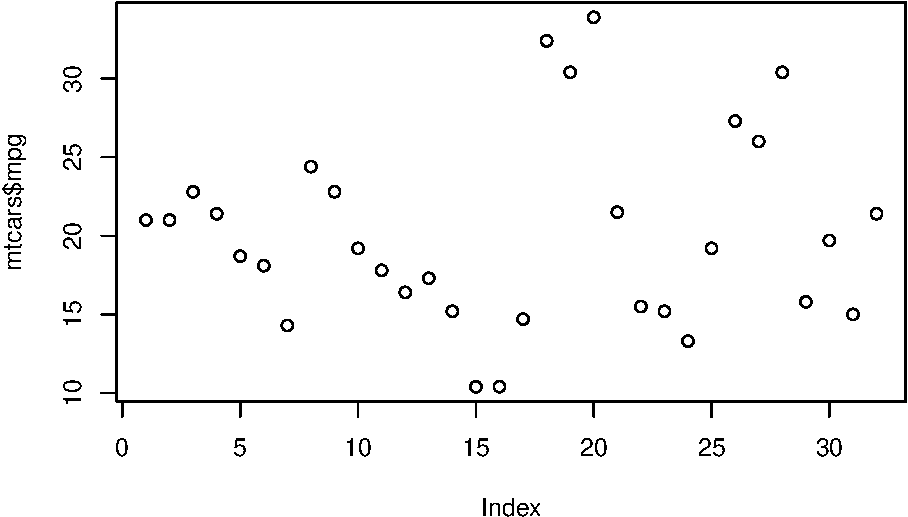
\includegraphics{01-rmarkdown-paper-pdf_files/figure-latex/unnamed-chunk-1-1.pdf}

\hypertarget{tables}{%
\subsection{Tables}\label{tables}}

\lipsum[12]

See awesome Table\textasciitilde{}\ref{tab:table}.

\begin{table}
 \caption{Sample table title}
  \centering
  \begin{tabular}{lll}
    \toprule
    \multicolumn{2}{c}{Part}                   \\
    \cmidrule(r){1-2}
    Name     & Description     & Size ($\mu$m) \\
    \midrule
    Dendrite & Input terminal  & $\sim$100     \\
    Axon     & Output terminal & $\sim$10      \\
    Soma     & Cell body       & up to $10^6$  \\
    \bottomrule
  \end{tabular}
  \label{tab:table}
\end{table}

\hypertarget{lists}{%
\subsection{Lists}\label{lists}}

\begin{itemize}
\tightlist
\item
  Lorem ipsum dolor sit amet
\item
  consectetur adipiscing elit.
\item
  Aliquam dignissim blandit est, in dictum tortor gravida eget. In ac
  rutrum magna.
\end{itemize}

\hypertarget{refs}{}
\begin{CSLReferences}{1}{0}
\leavevmode\hypertarget{ref-hadash2018estimate}{}%
Hadash, Guy, Einat Kermany, Boaz Carmeli, Ofer Lavi, George Kour, and
Alon Jacovi. 2018. {``Estimate and Replace: A Novel Approach to
Integrating Deep Neural Networks with Existing Applications.''}
\emph{arXiv Preprint arXiv:1804.09028}.

\leavevmode\hypertarget{ref-kour2014fast}{}%
Kour, George, and Raid Saabne. 2014a. {``Fast Classification of
Handwritten on-Line Arabic Characters.''} In \emph{Soft Computing and
Pattern Recognition (SoCPaR), 2014 6th International Conference of},
312--18. IEEE.

\leavevmode\hypertarget{ref-kour2014real}{}%
---------. 2014b. {``Real-Time Segmentation of on-Line Handwritten
Arabic Script.''} In \emph{Frontiers in Handwriting Recognition (ICFHR),
2014 14th International Conference on}, 417--22. IEEE.

\end{CSLReferences}

\bibliographystyle{unsrt}
\bibliography{references.bib}


\end{document}
